\chapter{Planificación completa}
\label{chap:planificacion-completa}

%%%%%%%%%%%%%%%%%%%%%%%%%%%%%%%%%%%%%%%%%%%%%%%%%%%%%%%%%%%%%%%%%%%%%%%%%%%%%%%%
% Objetivo: Lista de términos utilizados en el documento,                      %
%           junto con sus respectivos significados.                            %
%%%%%%%%%%%%%%%%%%%%%%%%%%%%%%%%%%%%%%%%%%%%%%%%%%%%%%%%%%%%%%%%%%%%%%%%%%%%%%%%

\lettrine{N}{este} apéndice exponse a planificación completa do proxecto que,
dada a súa extensión, non é posible incluír intercalada no correspondente
apartado da memoria.

\section{Planificación inicial}

A continuación exponse a planificación inicial con dependencias entre tarefas
incluídas e en orde cronolóxica (figuras
\ref{figura:PlanificacionInicialCompleta1} a
\ref{figura:PlanificacionInicialCompleta8}). \\

Na seguinte ligazón disponse da planificación inicial completa en alta
resolución: \\

\url{http://initialplanning.proxecto-puding.org} \\

\begin{figure}
 \centering
 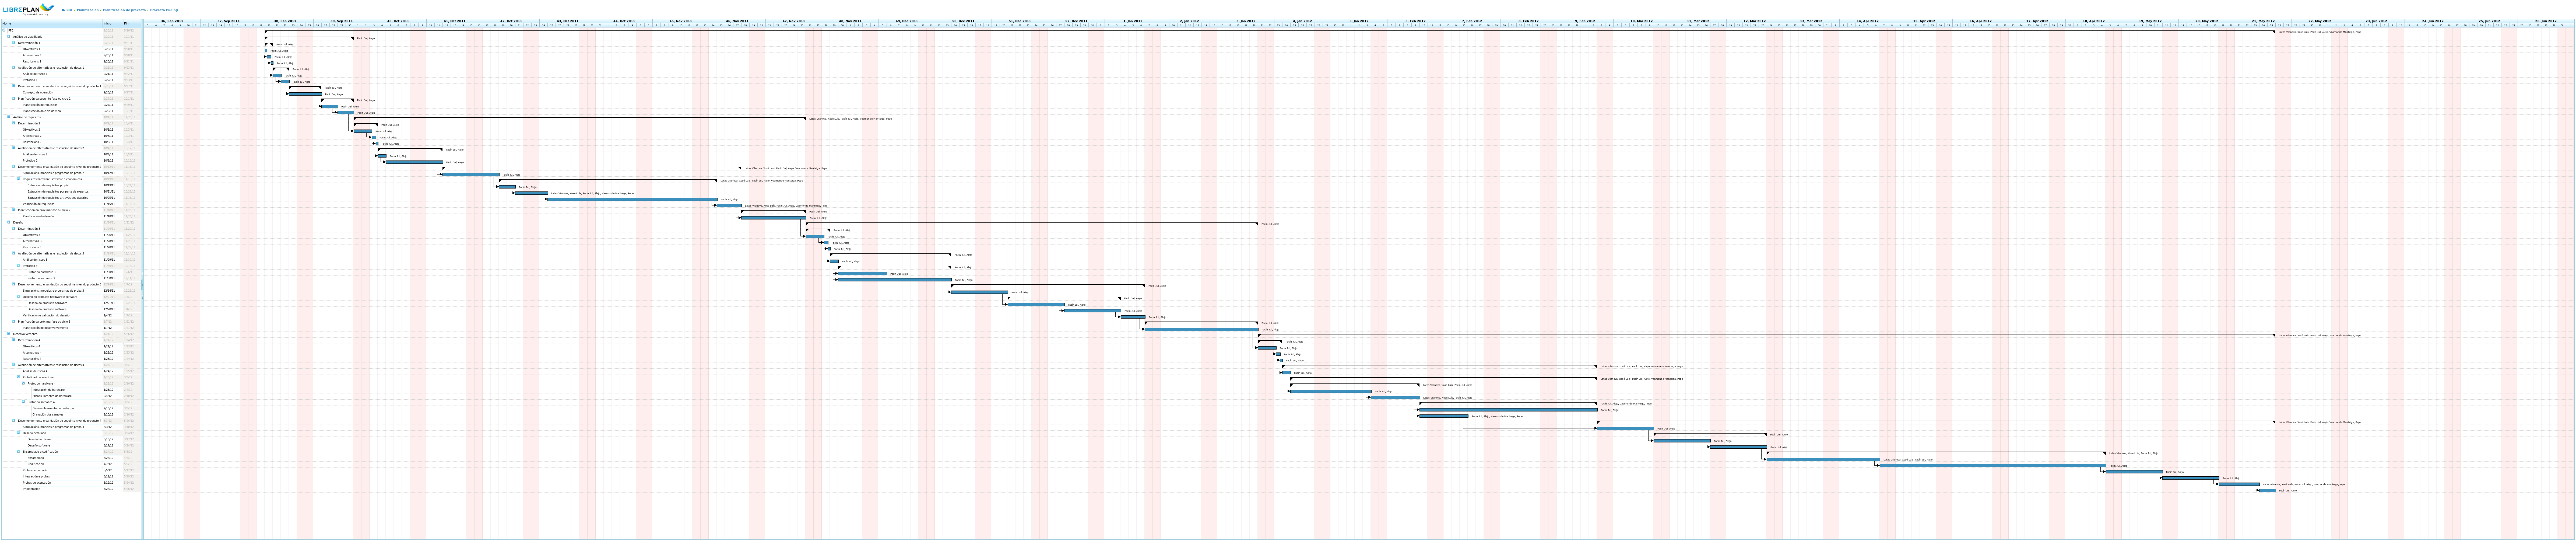
\includegraphics[trim=0 5cm 213cm 0,clip=true,scale=0.45,keepaspectratio=true]{./imagenes/planificacion-inicial.png}
 % enquisa.pdf: 612x792 pixel, 72dpi, 21.59x27.94 cm, bb=0 0 612 792
 \caption{Planificación inicial (p. 1)}
 \label{figura:PlanificacionInicialCompleta1}
\end{figure}

\begin{figure}
 \centering
 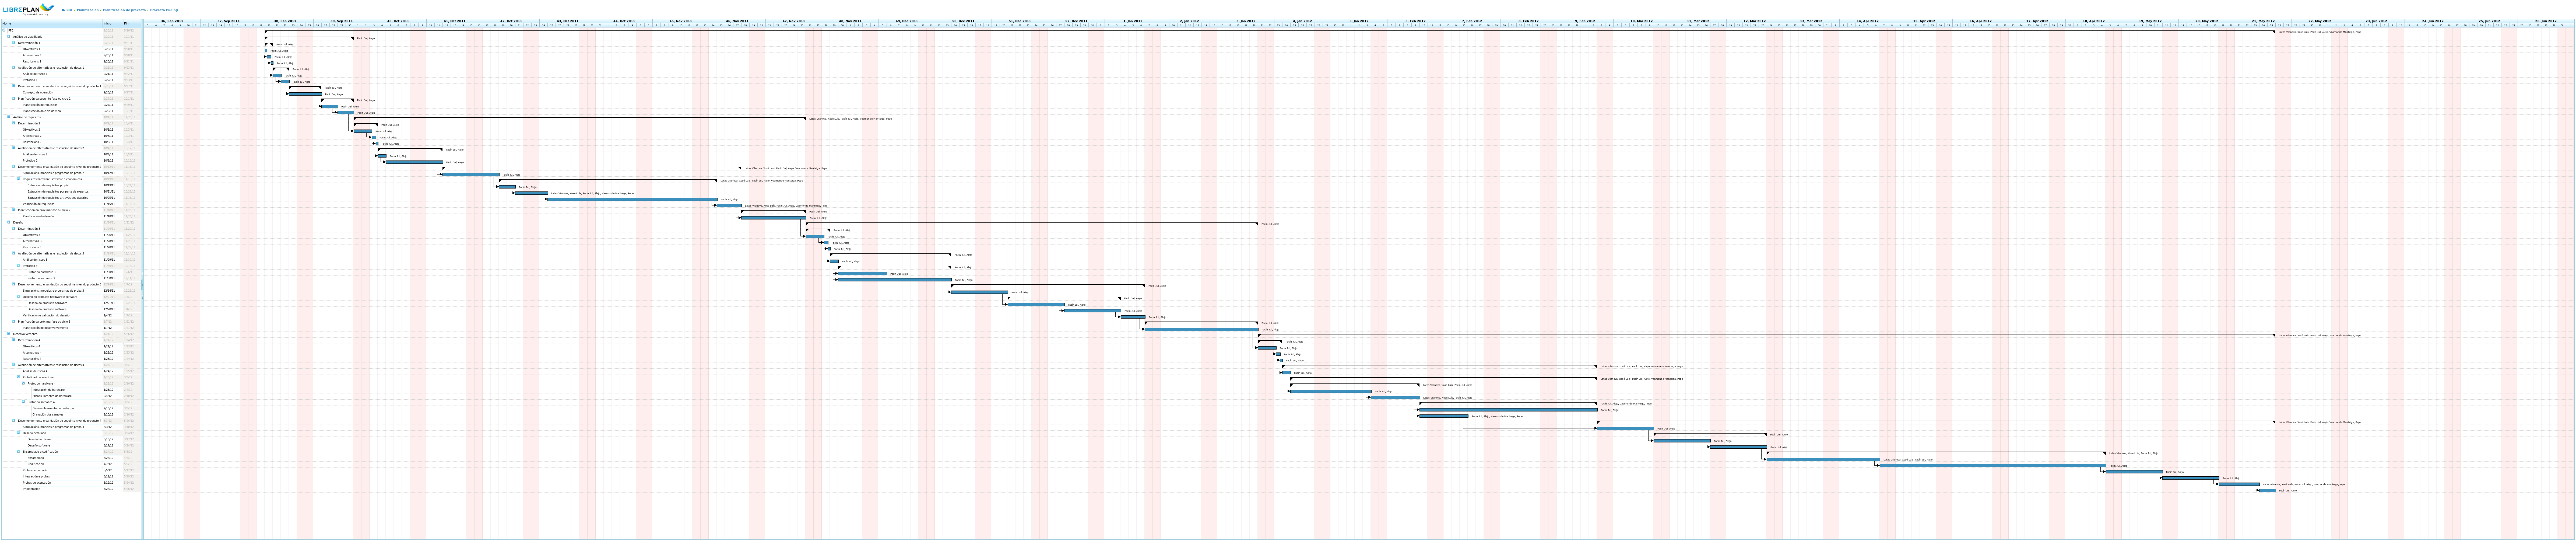
\includegraphics[trim=29cm 5cm 181cm 0,clip=true,scale=0.45,keepaspectratio=true]{./imagenes/planificacion-inicial.png}
 % enquisa.pdf: 612x792 pixel, 72dpi, 21.59x27.94 cm, bb=0 0 612 792
 \caption{Planificación inicial (p. 2)}
 \label{figura:PlanificacionInicialCompleta2}
\end{figure}

\begin{figure}
 \centering
 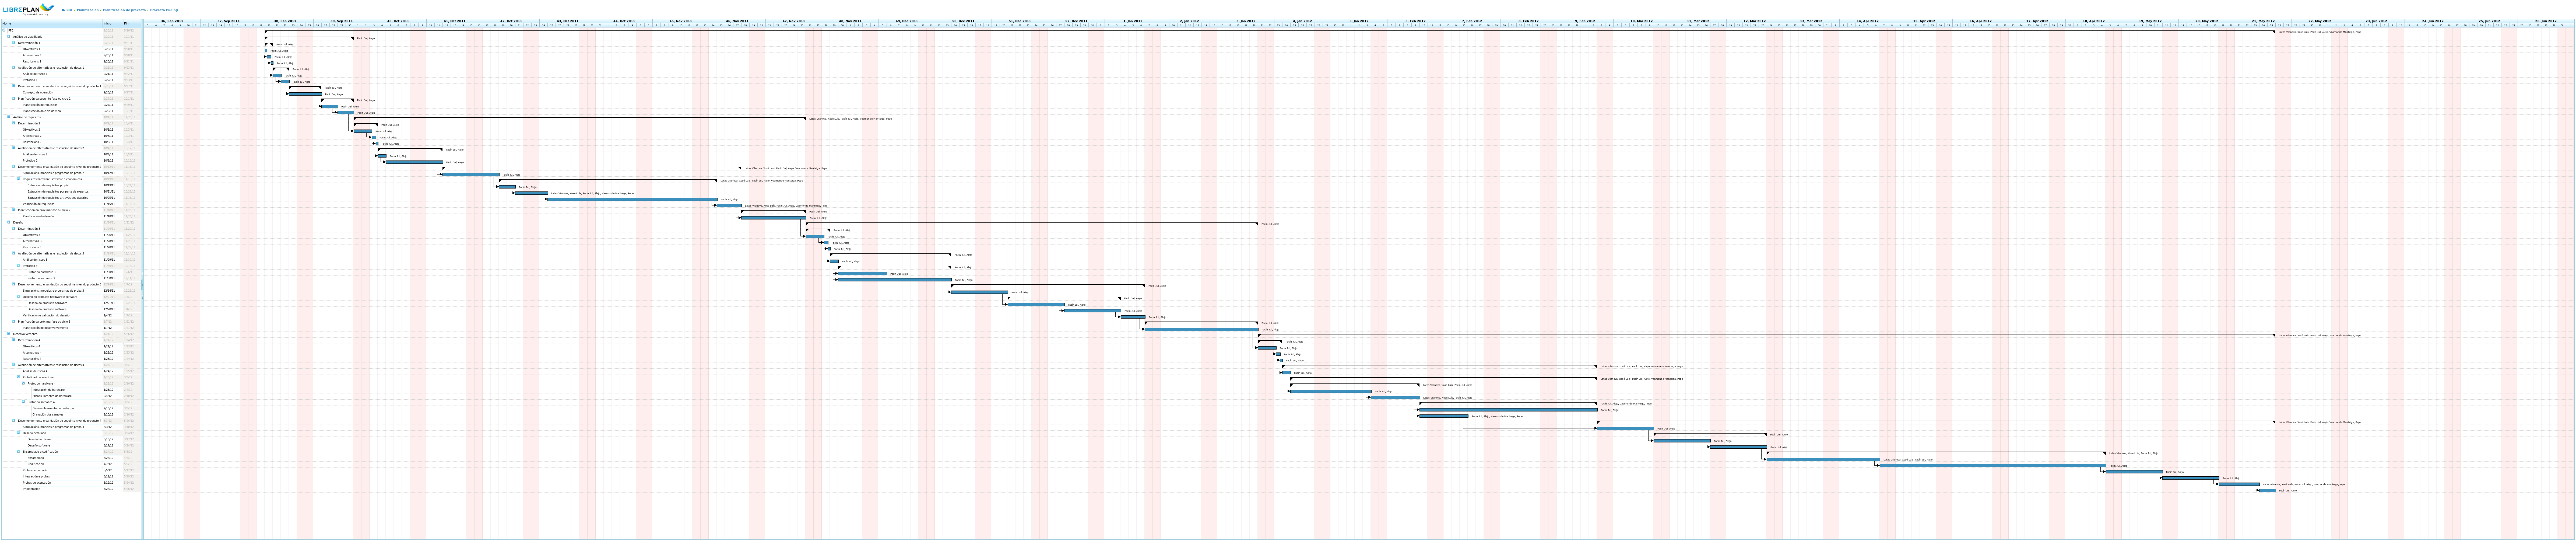
\includegraphics[trim=61cm 5cm 149cm 0,clip=true,scale=0.45,keepaspectratio=true]{./imagenes/planificacion-inicial.png}
 % enquisa.pdf: 612x792 pixel, 72dpi, 21.59x27.94 cm, bb=0 0 612 792
 \caption{Planificación inicial (p. 3)}
 \label{figura:PlanificacionInicialCompleta3}
\end{figure}

\begin{figure}
 \centering
 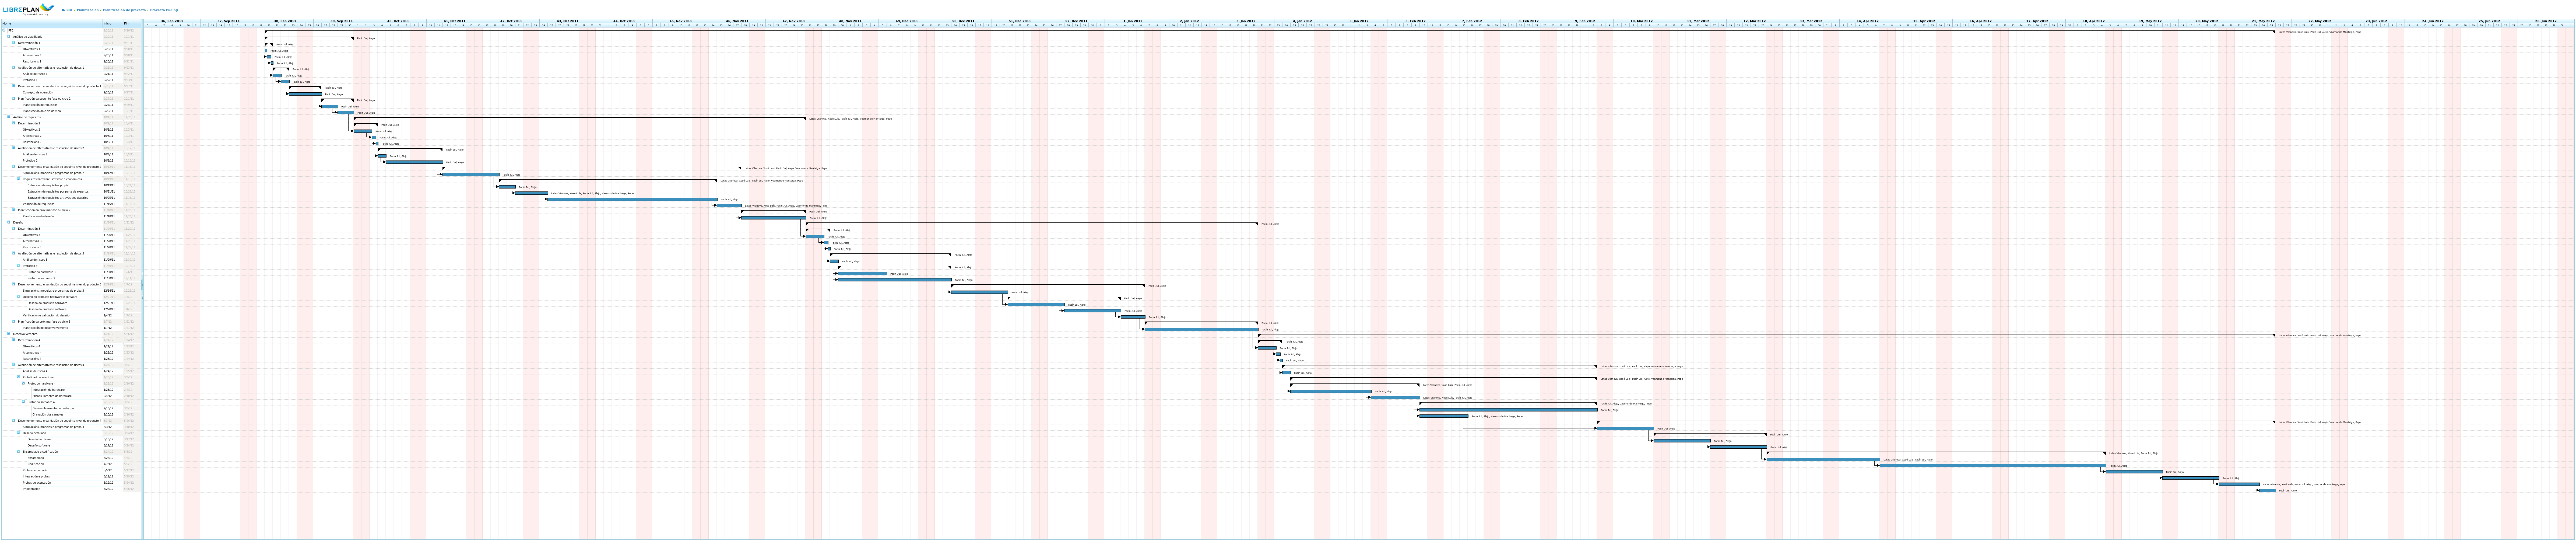
\includegraphics[trim=93cm 5cm 117cm 0,clip=true,scale=0.45,keepaspectratio=true]{./imagenes/planificacion-inicial.png}
 % enquisa.pdf: 612x792 pixel, 72dpi, 21.59x27.94 cm, bb=0 0 612 792
 \caption{Planificación inicial (p. 4)}
 \label{figura:PlanificacionInicialCompleta4}
\end{figure}

\begin{figure}
 \centering
 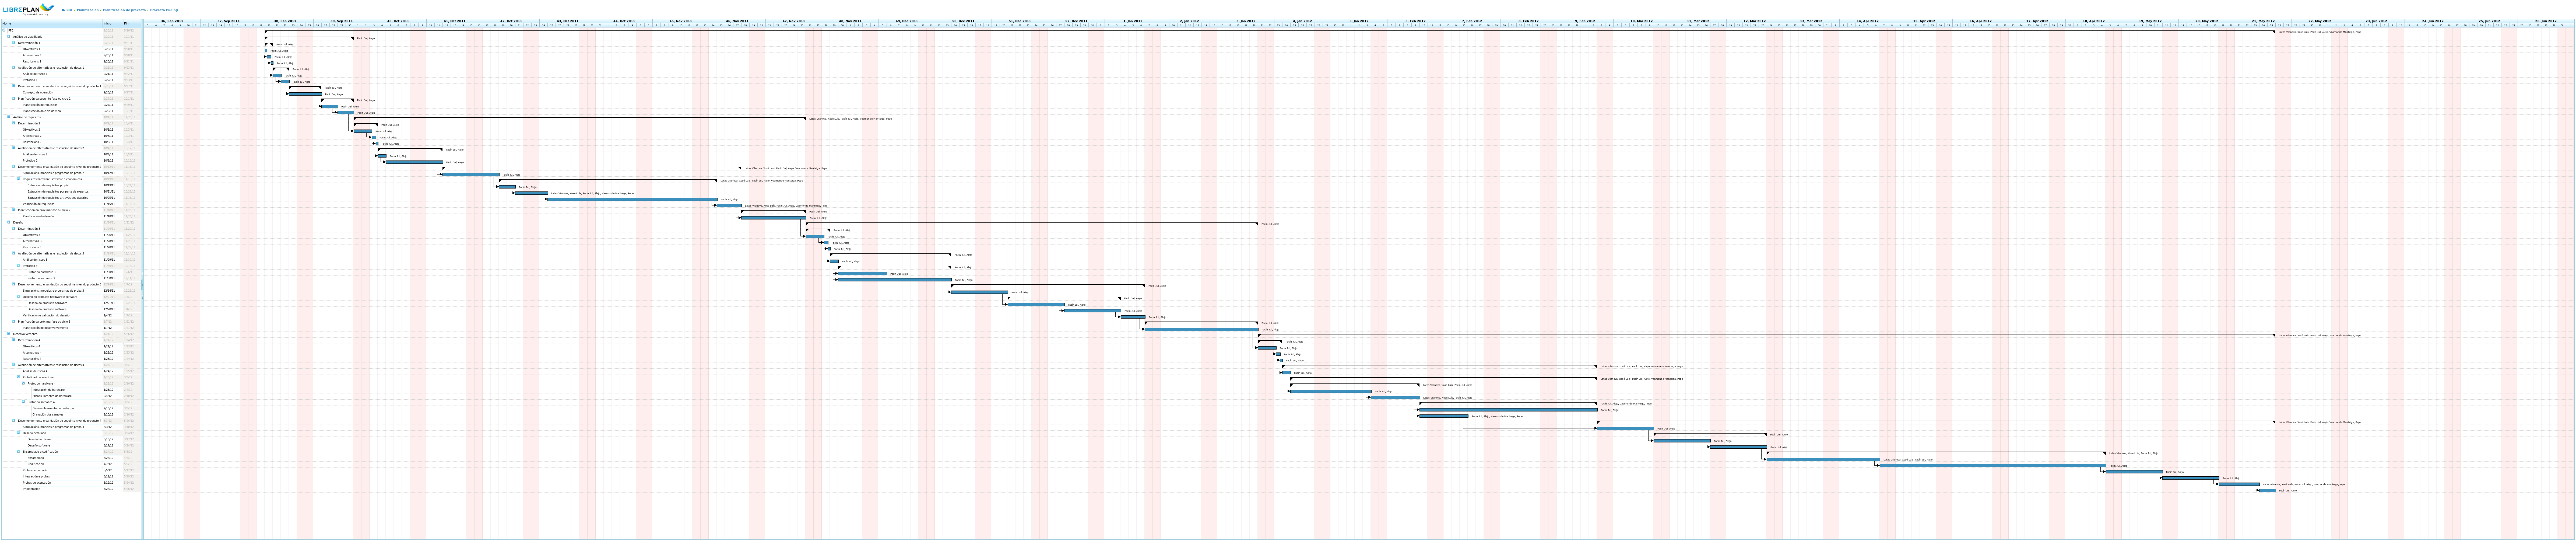
\includegraphics[trim=125cm 5cm 85cm 0,clip=true,scale=0.45,keepaspectratio=true]{./imagenes/planificacion-inicial.png}
 % enquisa.pdf: 612x792 pixel, 72dpi, 21.59x27.94 cm, bb=0 0 612 792
 \caption{Planificación inicial (p. 5)}
 \label{figura:PlanificacionInicialCompleta5}
\end{figure}

\begin{figure}
 \centering
 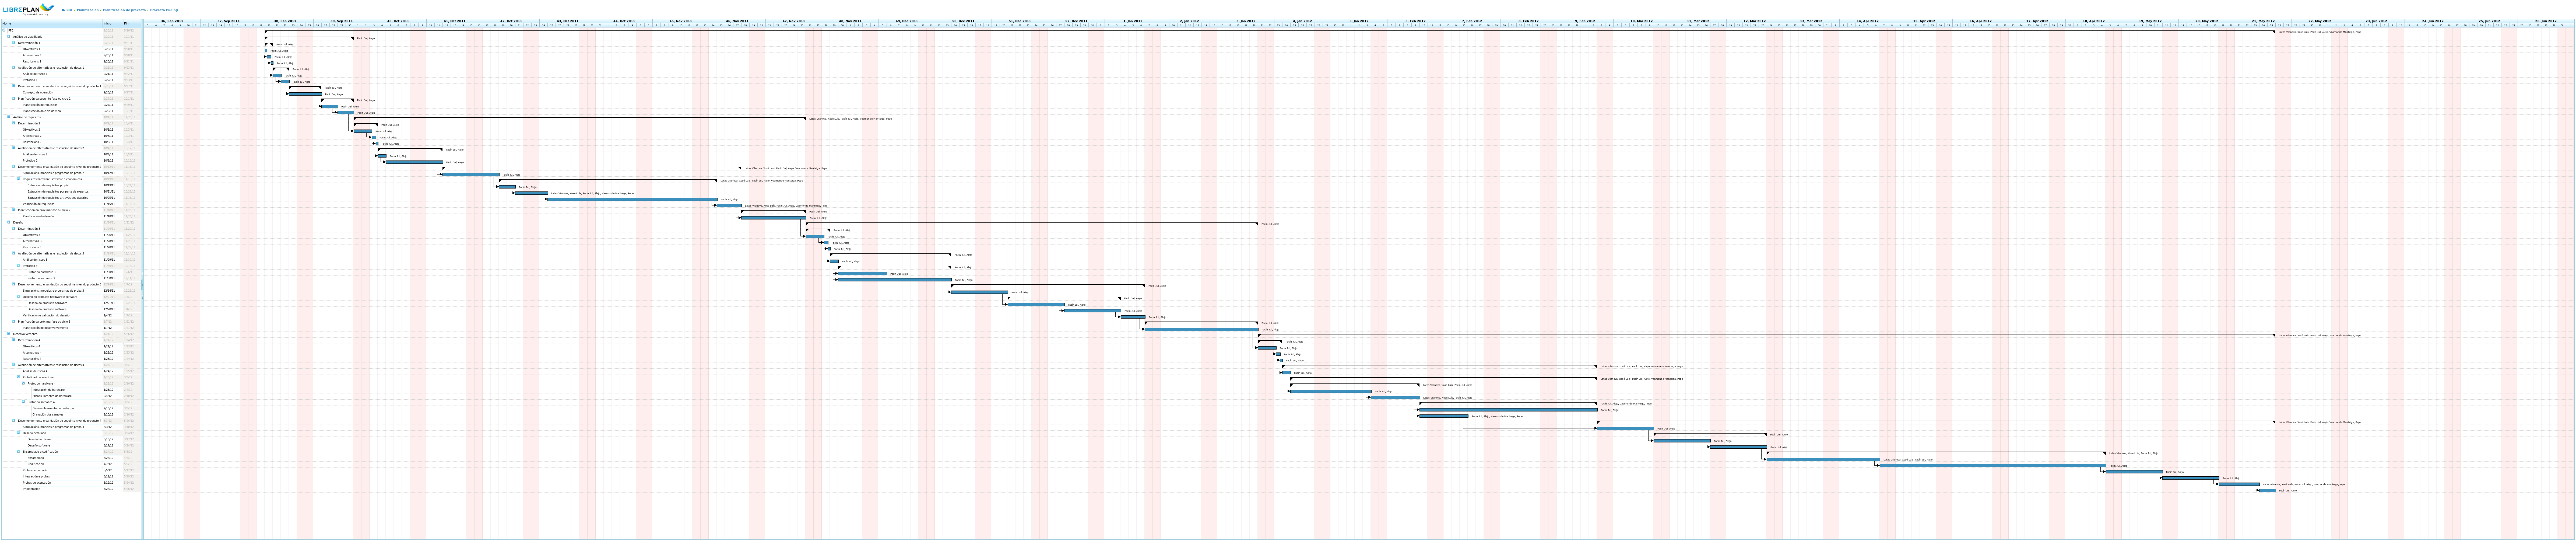
\includegraphics[trim=157cm 5cm 53cm 0,clip=true,scale=0.45,keepaspectratio=true]{./imagenes/planificacion-inicial.png}
 % enquisa.pdf: 612x792 pixel, 72dpi, 21.59x27.94 cm, bb=0 0 612 792
 \caption{Planificación inicial (p. 6)}
 \label{figura:PlanificacionInicialCompleta6}
\end{figure}

\begin{figure}
 \centering
 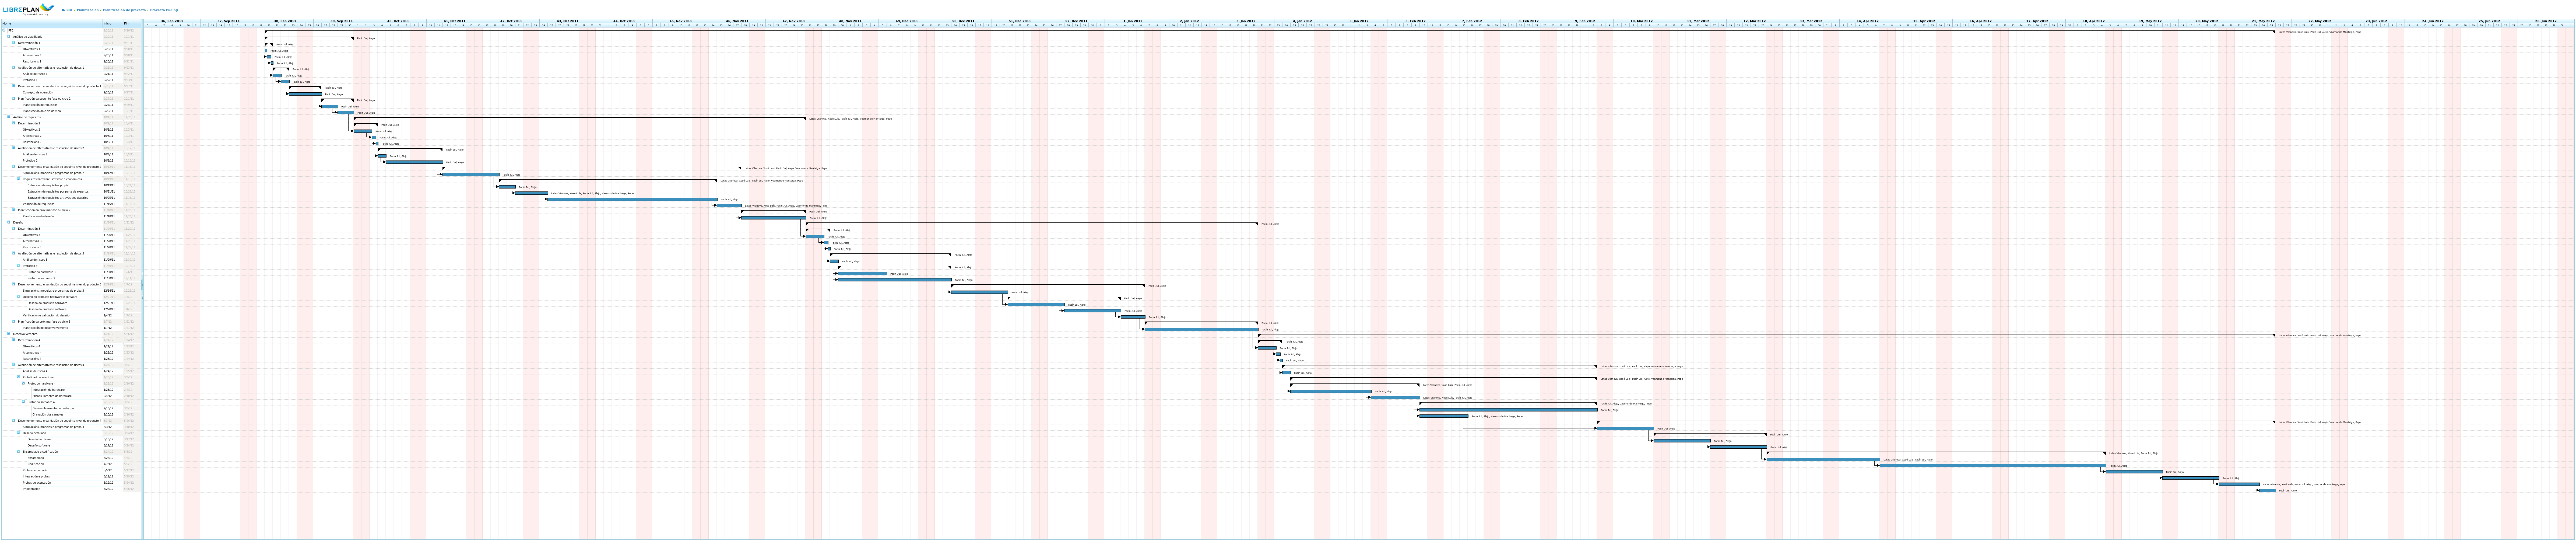
\includegraphics[trim=189cm 5cm 21cm 0,clip=true,scale=0.45,keepaspectratio=true]{./imagenes/planificacion-inicial.png}
 % enquisa.pdf: 612x792 pixel, 72dpi, 21.59x27.94 cm, bb=0 0 612 792
 \caption{Planificación inicial (p. 7)}
 \label{figura:PlanificacionInicialCompleta7}
\end{figure}

\begin{figure}
 \centering
 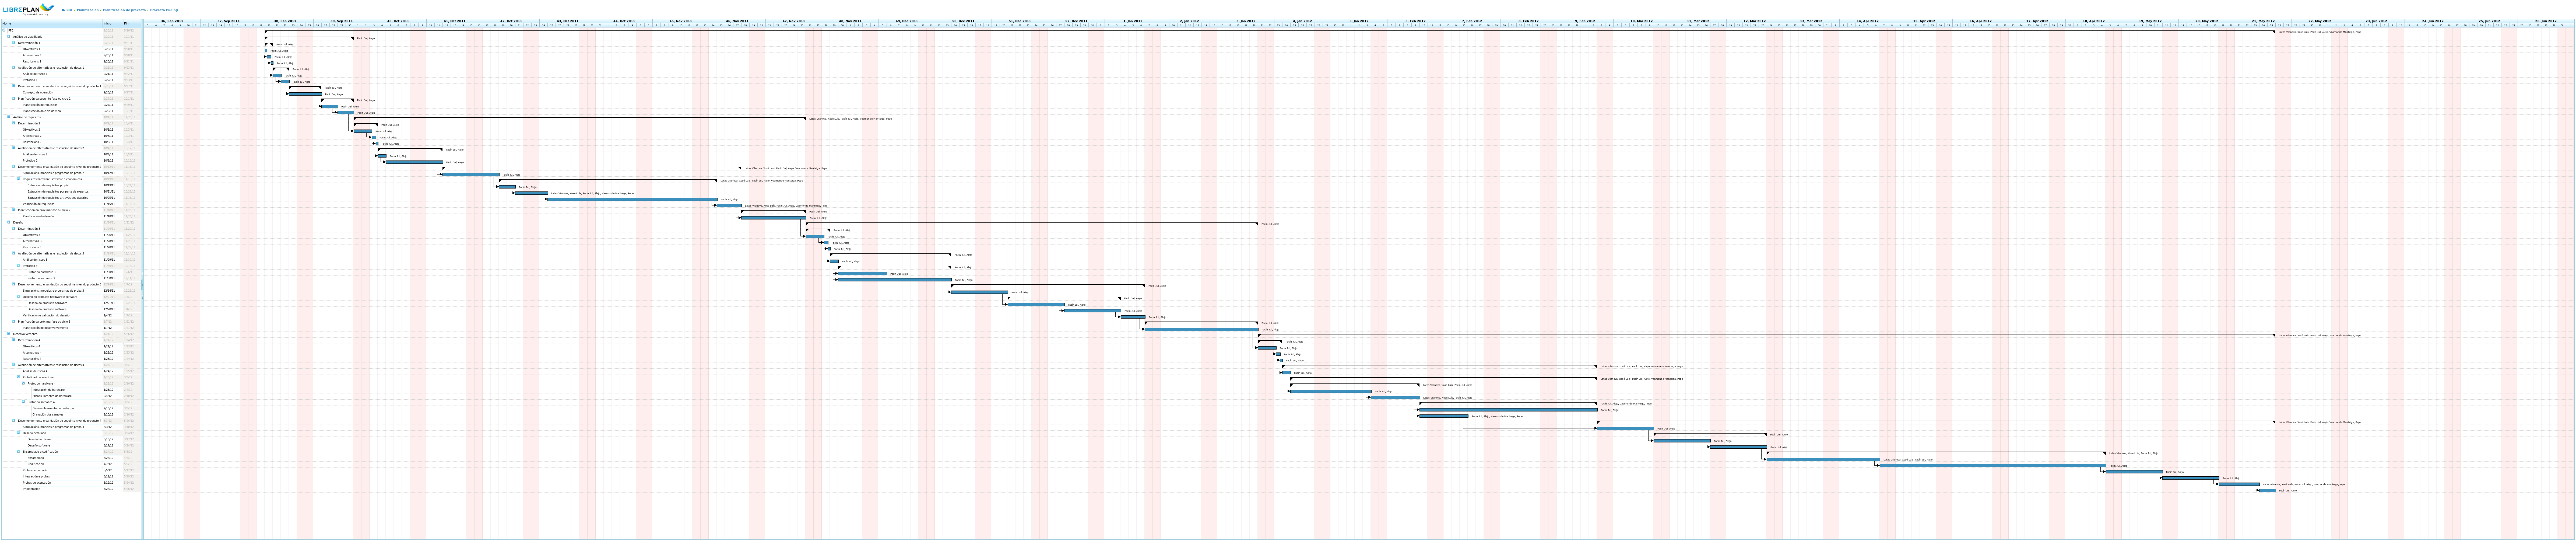
\includegraphics[trim=221cm 5cm 0 0,clip=true,scale=0.45,keepaspectratio=true]{./imagenes/planificacion-inicial.png}
 % enquisa.pdf: 612x792 pixel, 72dpi, 21.59x27.94 cm, bb=0 0 612 792
 \caption{Planificación inicial (p. 8)}
 \label{figura:PlanificacionInicialCompleta8}
\end{figure}

\section{Planificación final}

A continuación exponse a planificación final comparando as horas estimadas
contra as horas reais e seguindo a mesma orde que na planificación inicial
(figuras \ref{figura:PlanificacionFinal1} e \ref{figura:PlanificacionFinal1}). \\

Na seguinte ligazón disponse da planificación final completa en alta
resolución: \\

\url{http://finalplanning.proxecto-puding.org} \\

\begin{figure}[htbp]
 \centering
 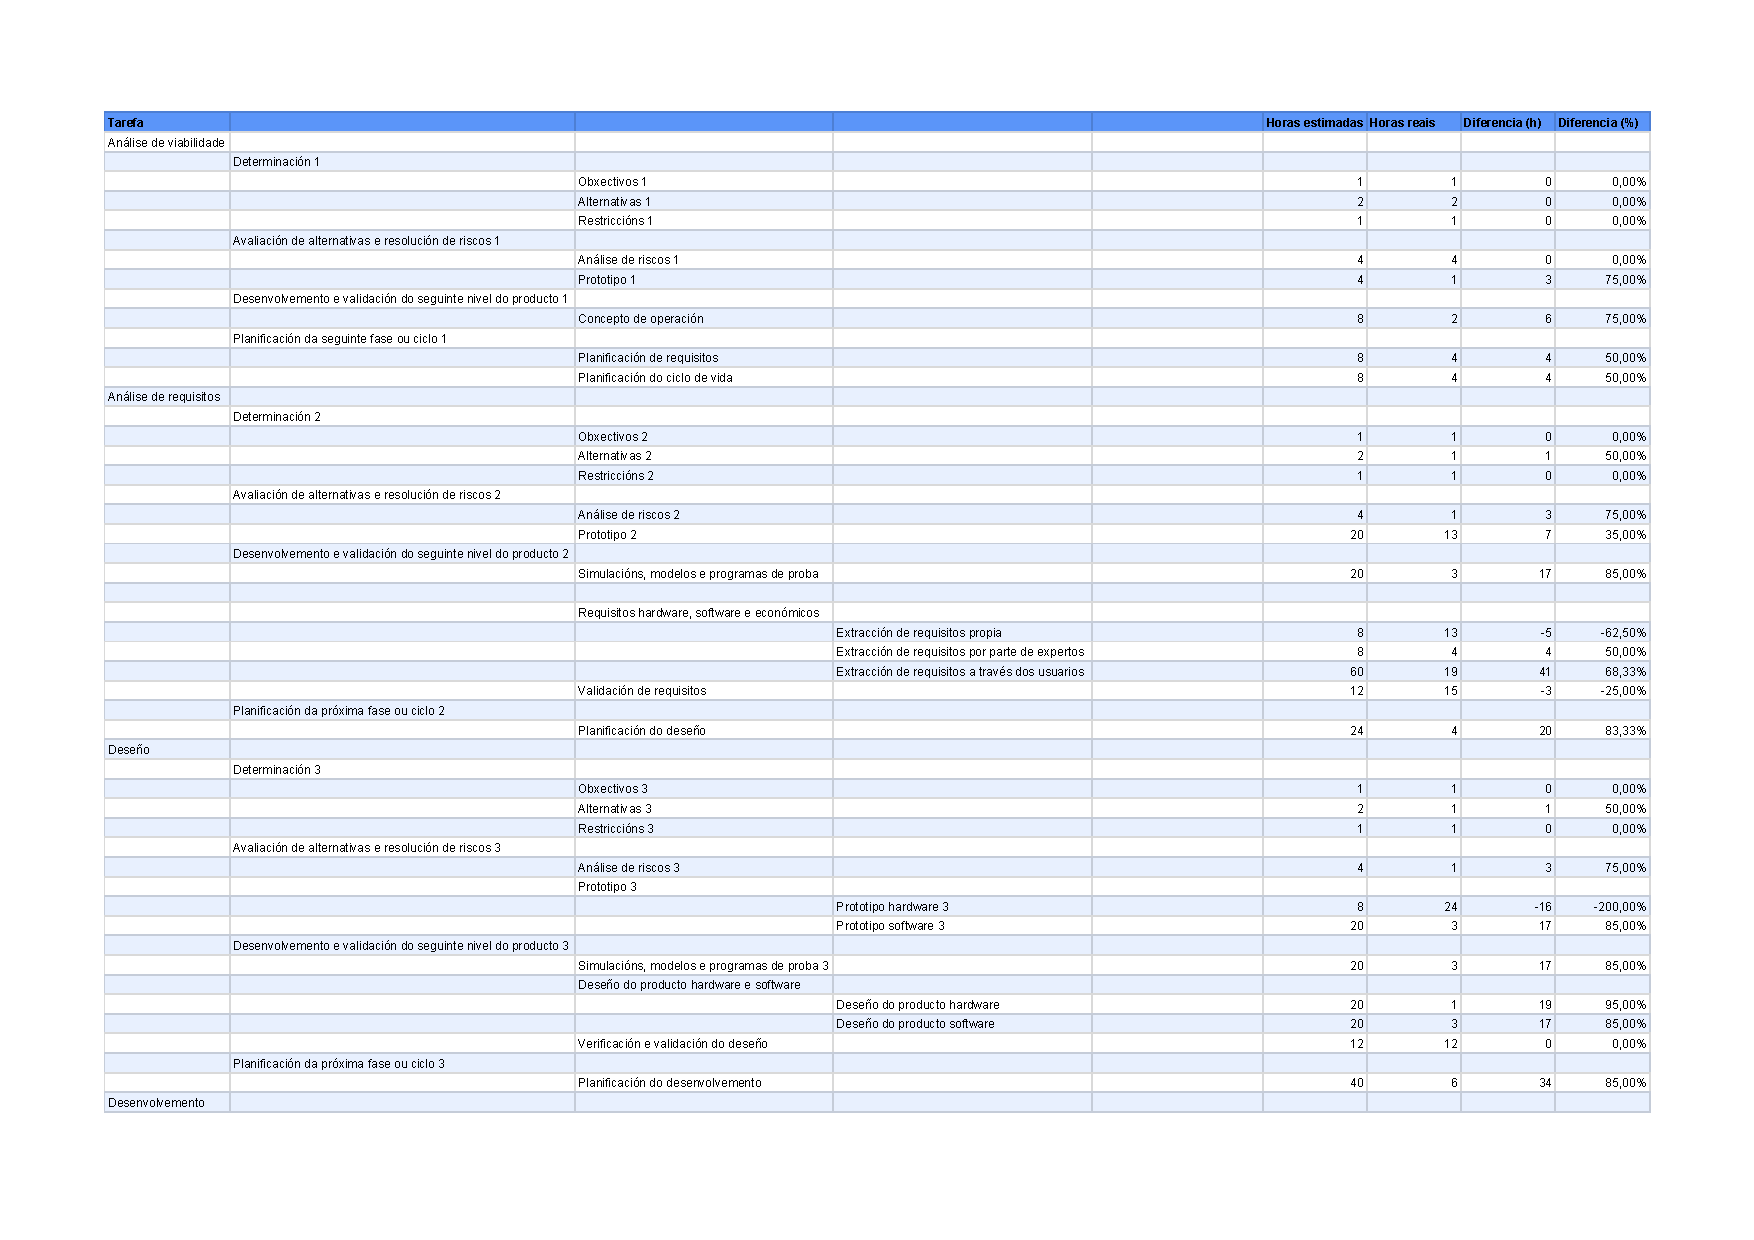
\includegraphics[scale=0.7,angle=90,page=1,keepaspectratio=true]{./imagenes/planificacion-final.pdf}
 % planificacion-final.pdf: 612x792 pixel, 72dpi, 21.59x27.94 cm, bb=0 0 612 792
 \caption{Planificación final (p. 1)}
 \label{figura:PlanificacionFinal1}
\end{figure}

\begin{figure}[htbp]
 \centering
 \includegraphics[scale=0.7,angle=90,page=2,keepaspectratio=true]{./imagenes/planificacion-final.pdf}
 % planificacion-final.pdf: 612x792 pixel, 72dpi, 21.59x27.94 cm, bb=0 0 612 792
 \caption{Planificación final (p. 2)}
 \label{figura:PlanificacionFinal2}
\end{figure}

Tal e como se pode apreciar nas imaxes, nas primeiras fases do proxecto
aforrouse algo máis dun 50\% das horas. \\

Foi na última fase, na de implementación e máis concretamente na última fase de
prototipado e máis na codificación final. Outras como o prototipo hardware da
fase de deseño ou os tests de integración tamén se foron moi arriba, pero
causaron menos impacto polo número de horas en relación ó total. \\

En xeral, sobreestimamos bastante o tempo necesario para as fases iniciais aínda
que non tiñan tanto impacto en horas e subestimamos moito as tarefas de
codificación, que si tiveron un impacto moi alto. \\

Como se pode apreciar, finalmente o total de horas ascendeu a 966 fronte ás 688
horas estimadas inicialmente, cunha desviación total contraria do 40\%. Unha
desviación alta se o consideramos un proxecto clásico de enxeñería, pero
comprensible polo alto compoñente de incertidume como proxecto de I+D puro. \\
